Above we study CFT on a complex plane or a Cylinder. How, we nay focus on more bizarre situation, CFT with boundaries, which is called Boundary Conformal Field Theory (BCFT). 

\subsection{General Picture of BCFT}

\axm{
  \textbf{General Picture of BCFT}

  The construction of BCFT is induced from a ordinary CFT. We consider given a CFT defined on a plane. We call it the \textbf{Parent CFT}. Then we chop off a setionand make a boundary. We consider what is the behaiour of the theory\dots

  Note that inducing a parent CFT to a BCFT is never unique. Different boundary conditions may lead to different theories. 
}


\subsubsection{BCFT on Upper Half Plane}

In General we can study BCFT on any kinds of Boundary, but here we focus on the simplest case, BCFT on Upper Half Plane (UHP) $ \mathbb{H} $. Considering UHP is general because of the Riemann Mapping Theorem:
\thm{
  \textbf{Riemann Mapping Theorem}

  Any simply connected open subset of the complex plane which is not the entire plane is conformally equivalent (exist a biholomophic map between) to the open unit disk:
  \begin{align}
    D=\{z\in\mathbb{C}:|z|<1\}
  \end{align}
}
And we can map the unit disk to UHP via a Mobius Transformation:
\begin{align}
  w=\frac{z-i}{z+i} \quad z \in \mathbb{H} ,  w \in \mathbb{D}.
\end{align}


\subsubsection{Conformal Transformation on UHP}

Then we analyze the conformal transformation on the UHP. Due to the existence of the boundary, not all holomorphic transformations are allowed, only those preserving the boundary are allowed. Thus, we have:
\defi{
  \textbf{Conformal Transformation on UHP}

  The conformal transformation on UHP are the holomorphic transformations $ \epsilon(z) $ satisfying:  
  \begin{align}
    \mathrm{Im}(\epsilon(z))=0 \quad \text{for } z \in \mathbb{R}
  \end{align}
}
\rmk{
  We also have to notice that now $ \epsilon(z) $ has its image and domain restricted to UHP $ \mathbb{H} $ only.
}
Thus as expected the conformal algebra of a boundary CFT should be smaller than the conformal algebra of a CFT without boundary. 

We often use a analytical continuation trick to reformulate the conformal transformation on UHP. We define:
\defi{
  \textbf{Analytical continued conformal transformation}

  The analytical continued conformal transformation $ \epsilon(z) $ on the whole complex plane is defined as:
  \begin{align}
    \epsilon^{H}(z) = \begin{cases}
      \epsilon(z) & \text{if } \mathrm{Im}(z) > 0 \\
      \bar{\epsilon}(z) & \text{if } \mathrm{Im}(z) < 0
    \end{cases}
  \end{align}
}
This is mathematically available because of the boundary condition $ \mathrm{Im}(\epsilon(z))=0 $ on the real axis.

\subsection{Conformal Boundary Conditions}

\subsubsection{General Boundary Conditions}

In ordinary QFT, if we have a boundary of the theory we need to fix a boundary condition. In ordinary QFT we have a dynamical field $ \phi $ with action $ S[\phi] $. 

Then what we can do is to fix a boundary condition for the dynamical field and we're done once and for all. We may take Dirichlet Boundary Condition (DBC) or Neumann Boundary Condition (NBC) or any other boundary condition we like:
\begin{align}
  & \text{DBC: } \phi|_{\partial M} = \phi_0, \\
  & \text{NBC: } \partial_n \phi|_{\partial M} = 0, 
\end{align}

\subsubsection{Conformal Boundary Condition}

In CFT, we only have the Primaries and Descendants. We can't tell what they should satisfy on the boundary for general discussion (However, if we can write a Lagrangian for CFT, we of course can write those fields with dynamical field and fix a boundary condition). Thus, we focus on what is generally consistent, one condition is that:
\begin{itemize}
  \item \textbf{Energy can't flow across the boundary}
\end{itemize}
Mathematically, if we consider the UHP then it is written as:
\defi{
  \textbf{Conformal Boundary Condition (Gluing Condition)}

  On the boundary of a CFT:
\begin{align}
  \int_{-\infty}^\infty dxT_{01}(x,0)=0
\end{align}
or we assume locally:
\begin{align}
  T_{01}(x,0)=0
\end{align}
or equivalently in the holomorphic and anti-holomorphic coordinates :
\begin{align}
  T(z)=\bar{T}(\bar{z}) \quad \text{on } z=\bar{z}
\end{align}
This is consistent with the definition \cref{eq:holomorphic EM tensor}.
}


\subsubsection{Boundary Conditions}

The Gluing Condition is never enough to define a CFT with boundary. Apparently, we need more information of the behavior of the fields on the boundary. 

For example, for a CFT with a lagrangian description, eg. the free boson CFT, we can have DBC or NBC for the dynamical field $ \phi $ on the boundary. These two boundary conditions will lead to different correlation functions and different physical behavior of the theory. Thus, apart from the Gluing Condition, we need more data to define a BCFT. Thus, we need some more conditions:

\defi{
  \textbf{Boundary Conditions in BCFT}

  We assume that consider a BCFT induced from a CFT, there exist a set of \textbf{boundary conditions} $ \{\alpha\} $ which consistently define the behavior of the fields.
}


\subsection{Ward Identities with Boundary}

We recall the conformal Ward identity \cref{axm:conformal ward identity}:
 \begin{align}
    \delta_{\epsilon,\bar{\epsilon}}\langle X\rangle=-\frac{1}{2\pi i}\oint_{C}dz\mathrm{~}\epsilon(z)\langle T(z)X\rangle-\frac{1}{2\pi i}\oint_{\bar{C}}d\bar{z}\mathrm{~}\bar{\epsilon}(\bar{z})\langle\bar{T}(\bar{z})X\rangle
 \end{align}
 \rmk{
   This Identity hold for any theory with conformal symmetry. When considering th e boundary, the only thing we need to change is:
   \begin{itemize}
     \item $ z $ can only take values in UHP and $ \bar{z} = z^* $ thus can only take values in LHP. 
     \item Transformation $ \epsilon(z) $ and $ \bar{\epsilon}(\bar{z}) $ must preserve the boundary. Thus, they can't be independent and we can't decouple the holomorphic and anti-holomorphic parts any more.
   \end{itemize}
 }
Before we use the decoupling trick to make the holomorphic and anti-holomorphic parts independent. Now, we can't do this trick because of the existence of boundary. Thus, we have to deal with the two parts together.
\subsubsection{Analytical Continuation Trick}

We focus on the E-M tensors $ T(z) $ and $ \bar{T}(\bar{z}) $ and $ z \in \text{UHP} , \bar{z} = z^* $. In fact we now don't need two independent E-M tensors defined on half of the complex plane, we can define a single E-M tensor on the whole complex plane to encode the information of both $ T(z) $ on the UHP and $ \bar{T}(\bar{z}) $ on LHP. 
\defi{
  \textbf{Analytical continued E-M Tensor}

  we define the analytical continued E-M tensor $ T(z) $ on the whole complex plane as:
  \begin{align}
    T^{H}(z) = \begin{cases}
      T(z) & \text{if } \mathrm{Im}(z) > 0 \\
      \bar{T}(z) & \text{if } \mathrm{Im}(z) < 0
    \end{cases}
  \end{align}
  This is a holomorphic function on $ \mathbb{C} $.
}
\rmk{
  Mathenatically, This is called the Analytic Continuation. And we can prove that this function is holomorphic on $ \mathbb{C} $ mathematically.
}
Just as what we do for the E-M tensor in normal CFT, we can mode expand the analytical continued E-M tensor:
\defi{
  \textbf{Mode Expansion of Analytical continued E-M Tensor}

  The mode expansion of the analytical continued E-M tensor is defined as:
  \begin{align}
    T^{H}(z) = \sum_{n \in \mathbb{Z}} z^{-n-2} L_n^{H} , \quad L_n^{H} = \frac{1}{2\pi i} \oint_{C} dz z^{n+1} T^{H}(z)
  \end{align}
}
\rmk{
  Note that though we use the same notation of $ L_0 $ it is the mode expansion of the analytical continued E-M tensor now not just the holomorphic E-M tensor, but a combination of both holomorphic and anti-holomorphic E-M tensors.
}

\subsubsection{Conformal Ward Identity on UHP}

Thus, taking an appropriate contour shown in \cref{fig:newontour} the RHS of the conformal Ward Identity can we written as following:
\begin{align}
  RHS = - \oint_{C^+} \frac{dz}{2\pi i} \epsilon(z) \langle T(z) X \rangle_H - \oint_{\bar{C}^+} \frac{d\bar{z}}{2\pi i} \bar{\epsilon}(\bar{z}) \langle \bar{T}(\bar{z}) X \rangle_H = - \oint_{C^++\bar{C}^+} \frac{dz}{2\pi i} \epsilon^H(z) \langle T^H(z) X \rangle_H
\end{align}
\begin{figure}[H]
  \centering
  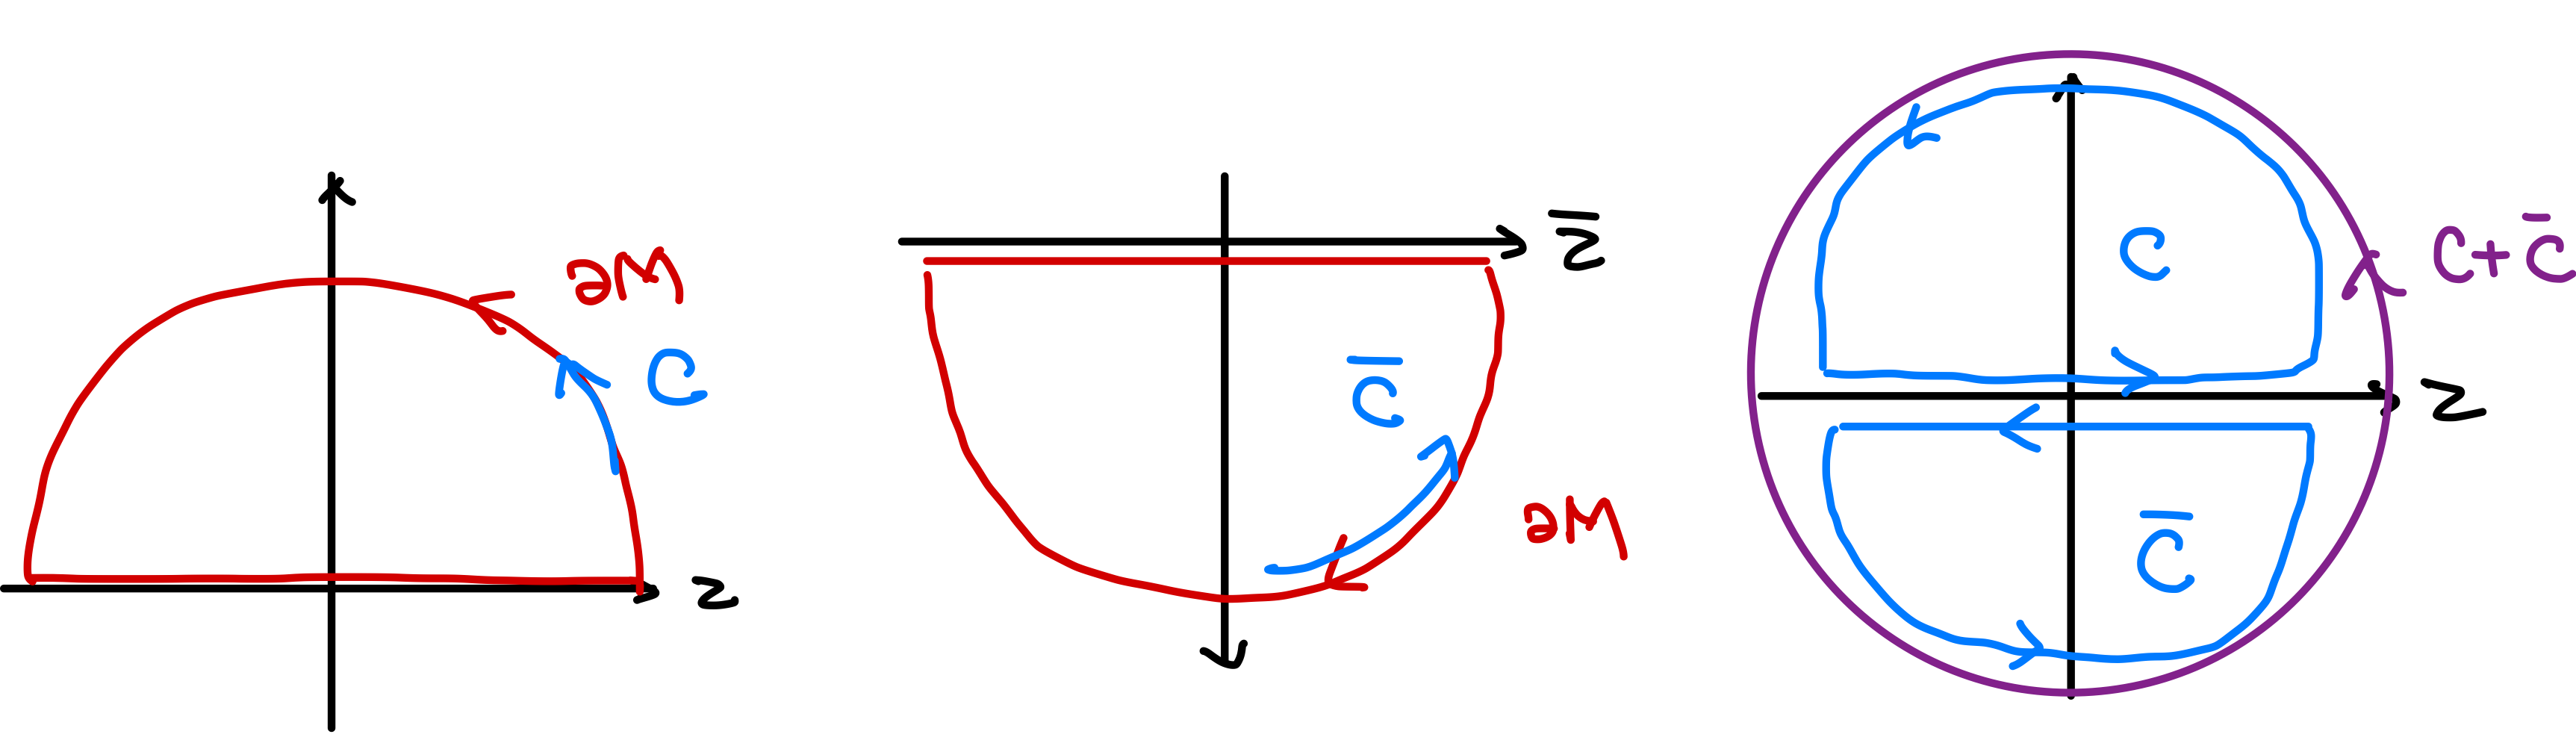
\includegraphics[width=0.75\textwidth]{assets/newontour.png}
  \caption{Choice of contour for conformal Ward identity on UHP after analytic continuation.}
  \label{fig:newontour}
\end{figure}
For Primary Field we can also do a similar trick to the LHS of the conformal Ward identity. We have:
\begin{align}
  LHS=&-\frac{1}{2\pi i}\oint_{C^+}dw\mathrm{~}\epsilon(w)\sum_{i=1}^n\left[\frac{1}{w-z_i}\partial_{z_i}+\frac{h_i}{(w-z_i)^2}\right]\langle X\rangle_H\\
      &-\frac{1}{2\pi i}\oint_{\bar{C}^+}d\bar{w}\mathrm{~}\bar{\epsilon}(\bar{w})\sum_{i=1}^n\left[\frac{1}{\bar{w}-\bar{z}_i}\partial_{\bar{z}_i}+\frac{\bar{h}_i}{(\bar{w}-\bar{z}_i)^2}\right]\langle X\rangle_H\\ 
  =&-\frac{1}{2\pi i}\oint_{C^++\bar{C}^+}dw\mathrm{~}\epsilon^H(w)\sum_{i=1}^n\left[\frac{1}{w-z_i}\partial_{z_i}+\frac{h_i}{(w-z_i)^2}+\frac{1}{w-\bar{z}_i}\partial_{\bar{z}_i}+\frac{\bar{h}_i}{(w-\bar{z}_i)^2}\right]\langle X\rangle_H
\end{align}
Thus, we now have the conformal Ward identity on UHP:
\thm{
  \textbf{Conformal Ward Identity of Primaries on UHP}

  On UHP, for a set of primary fields $ X = \prod_{i=1}^n \phi_i(z_i,\bar{z}_i) $ , we have the conformal Ward identity:
  \begin{align}
    \langle T^H(z) X \rangle_{H} = \sum_{i=1}^n \left[ \frac{1}{z - z_i} \partial_{z_i} + \frac{h_i}{(z - z_i)^2} + \frac{1}{z - \bar{z}_i} \partial_{\bar{z}_i} + \frac{\bar{h}_i}{(z - \bar{z}_i)^2} \right] \langle X \rangle_{H}
  \end{align}
  where $ z \in \mathbb{C} $ and $ T(z) $ is the analytical continued E-M tensor.
}
\rmk{
  Attention that on the above equation $ z_i  \in \text{UHP} $ however, $ z \in \mathbb{C} $. they have different domains.
}
Additionally, we can also assume the conformal Ward identity holds for more general fields beyond primaries on UHP as well:
\axm{\label{axm:conformal ward identity UHP}
  \textbf{Conformal Ward Identity on UHP}

  On UHP, for a general set of fields $ X $, we have the conformal Ward identity:
  \begin{align}
    \delta_{\epsilon^H} \langle X \rangle_{H} = - \displaystyle\frac{1}{2 \pi i} \oint_{C^++\bar{C}^+} \epsilon^H(z) \langle T^H(z) X \rangle_{H} 
  \end{align}
  where $ z \in \mathbb{C} $ and $ T^H(z) $ is the analytical continued E-M tensor.
}


\subsection{The Method of Images (Doubling Trick)}\label{sec:Method of Images}


The above discussion have give us a hint that the coorelation on the UHP bahave as if we have twice the number of fields on the whole complex plane. We observe the difference between the whole conformal Ward identity on UHP and the holomorphic conformal ward identity on the whole complex plane for primary fields:
\begin{align}
  \langle T(z) X_0 \rangle_{\mathbb{C}}& = \sum_{i=1}^n \left[ \frac{1}{z - z_i} \partial_{z_i} + \frac{h_i}{(z - z_i)^2} + \frac{1}{z - \bar{z}_i} \partial_{\bar{z}_i} + \frac{\bar{h}_i}{(z - \bar{z}_i)^2}\right] \langle X_0 \rangle_{\mathbb{C}}\\ 
  \langle T^H(z) X \rangle_{H} &= \sum_{i=1}^n \left[ \frac{1}{z - z_i} \partial_{z_i} + \frac{h_i}{(z - z_i)^2} + \frac{1}{z - \bar{z}_i} \partial_{\bar{z}_i} + \frac{\bar{h}_i}{(z - \bar{z}_i)^2}\right] \langle X \rangle_{H}
\end{align}
Where we have:
\begin{align}
  X_0 &= \prod_{i=1}^n \phi_i(z_i) \prod_{i=1}^n \bar{\phi}_i(\bar{z}_i), \quad z_i , \bar{z}_i \in \mathbb{C} , z_i^* = \bar{z}_i \\
  X &= \prod_{i=1}^n \phi_i(z_i,\bar{z}_i) , \quad z_i \in \text{UHP} , \bar{z}_i = z_i^* \in \text{LHP}
\end{align}
Where $ \phi_i(z_i) $ are chiral fields with conformal dimension $ (h_i,0) $ and $ \bar{\phi}_i(\bar{z}_i) $ are anti-chiral fields with conformal dimension $ (\bar{h}_i, 0) $. We assume that they are all holomorphic fields.
\begin{itemize}
  \item We can see that the \textbf{correlation function of the primaries on the UHP} satisfies the same differential equations as the \textbf{correlation function of twice of the number of chiral holomorphic fields on the whole complex plane}.
\end{itemize}
\rmk{
  By the word "chiral holomorphic fields" we mean the fields with conformal dimension $ (h,0) $ only and depends only on $ z $.

  In fact, chiral holomorphic fields can be physical, for example the majorana fermion field $ \phi(z) $ can be a $ (1/2,0) $ chiral holomorphic field.
}

By the procudure discussed in \cref{sec:CFT Correlation Functions}, we know that the correlation function are determined by solving the conformal ward identities. Thus, we can conclude that:
\thm{
  \textbf{Method of Images (Doubling Trick)}

  The \textbf{correlation function} of a set of primary fields $ X = \prod_{i=1}^n \phi_i(z_i,\bar{z}_i) $ on UHP 
  \[
    =
  \]
  $ \sum $ of the \textbf{chiral conformal blocks} of twice the number of chiral holomorphic fields $ X_0 = \prod_{i=1}^n \phi_i(z_i) \prod_{i=1}^n \bar{\phi}_i(\bar{z}_i) $ on the whole complex plane. 
}
Proof: this is a straightforward result of the definition of conformal blocks and the above discussion.

An example is that the 1-point correlation function on UHP can be computed via the 2-point chiral conformal blocks on the whole complex plane:
\begin{align}
  \langle \phi(z,\bar{z}) \rangle_{H} = \langle \phi(z) \bar{\phi}(\bar{z}) \rangle_{\mathbb{C}} \sim \frac{1}{(z - \bar{z})^{2h}} \text{ for } h = \bar{h}
\end{align}
There will be some constant prefactor to be determined by the theory and the boundary condition on the boundary.


\subsection{Canonical Quantization and Generators}

In the context of BCFT, we can also perform the Radial Quantization. However, the equal-time slices are now semi-circles instead of full circles due to the presence of the boundary. Other tahn this the strategy of canonical quantization is similar to the ordinary CFT:
\begin{itemize}
  \item Radial Ordering
  \item OPE and Commutators relation
    ...
\end{itemize}

\subsubsection{Hamiltonian on a semi-circle}
We first Consider the Hamiltonian on a semi-circle. We consider the integral on a semi-circle. We name the contour as $ S $ which is the semi-circle part of $ C^+ $ with the same orientation as $ C^+ $ and the contour $ \bar{S} $ which is the semi-circle part of $ \bar{C}^+ $ with the opposite orientation as $ \bar{C}^+ $. Then we have:

\defi{
  \textbf{Hamiltonian on Semi-circle}

  The Hamiltonian on a semi-circle is defined as:
  \begin{align}
    H^H =& \frac{1}{2\pi i} \oint_{S} dz\  z T(z) + \frac{1}{2\pi i} \oint_{\bar{S}} d\bar{z}\  \bar{z} \bar{T}(\bar{z})\\ 
    =& \frac{1}{2\pi i} \oint_{S + \bar{S} = C} dz \ z T^H(z)\\ 
    =& L_0^H
  \end{align}
where $ L_0^H $ is the mode expansion of the analytical continued E-M tensor.
}
We will take this as a Hamiltonian of the BCFT.


\subsubsection{Symmetry Algebra with Boundary}

Then we start to study the symmetry algebra with boundary. We notice that from the general conformal Ward identity on UHP \cref{axm:conformal ward identity UHP}, and the relation between the commutators and the OPE, we then have:
\begin{align}
  \delta_{\epsilon^H} \phi(w,\bar{w}) = [Q_{\epsilon^H}, \phi(w,\bar{w})] = \oint_{C} \frac{dz}{2\pi i} \epsilon^H(z) T^H(z) \phi(w,\bar{w})
\end{align}
The integral contour is around the origin with both $ w $ and $ \bar{w} $ inside of it. Then we can expand $ \epsilon^H(z) $ and just as the ordinary CFT case we can give out the generators as:
\begin{align}
  L_n^H = \frac{1}{2\pi i} \oint_{C} dz \ z^{n+1} T^H(z) = \oint_{C^+} \frac{dz}{2\pi i} z^{n+1} T(z) + \oint_{\bar{C}^+} \frac{d\bar{z}}{2\pi i} \bar{z}^{n+1} \bar{T}(\bar{z})
\end{align}
Just as the ordinary CFT case, we can compute the commutators between these generators via the OPE of $ T^H(z) $ with itself. We have:
\thm{
  \textbf{Symmetry Algebra with Boundary}

  The generators $ L_n^H $ defined above satisfy the Virasoro Algebra:
\begin{align}
  [L_n^H, L_m^H] = (n - m) L_{n+m}^H + \frac{c}{12} n (n^2 - 1) \delta_{n+m,0}
\end{align}
}
We can see that now the symmetry algebra of the BCFT is just a single copy of the Virasoro Algebra instead of two copies as in ordinary CFT. 

\subsubsection{Hilbert Space Structure with Boundary}

Similarly, the Hilbert Space structure should take as the representation of a single copy of the Virasoro Algebra. Thus, we have:
\thm{
  \textbf{Hilbert Space Structure with Boundary}

  The Hilbert Space of the BCFT is spanned by the highest weight representations of a single copy of the Virasoro Algebra:
  \begin{align}
    \mathcal{H}_\alpha = \bigoplus_{h} n^{h}_\alpha \mathcal{V}_h
  \end{align}
  where $ n_h $ are non-negative integers indicating the multiplicity of the representation $ \mathcal{V}_h $ in the Hilbert Space. Here we use $ \alpha $ to indicate the boundary condition of the BCFT.
}
Then we expect to construct this Hilbert Space via acting operators on the vaccum state. However, we might face contraditions here, if we nively act a bulk primary field $ \phi(z,\bar{z}) $ on the vacuum state $ |0\rangle $, then it transforms as a representation of two copies of the Virasoro Algebra instead of a single copy. Thus, the state-operator correspondence seems to be less obvious here.


\subsection{Boundary Fields}

\subsubsection{Boundary Operators}

In section \cref{sec:Method of Images} we have seen that the one point correlation function on UHP can be computed via the two-point chiral conformal blocks on the whole complex plane. The correlation function of single bulk field behave divergence as it approaches the boundary. This phenomenon indicates that there may exist some new fields living on the boundary to interact with the bulk fields. 
\rmk{
  In QFT, we understand divergence by revealing hidden existence of new fields.
}
\defi{
  \textbf{Boundary Fields}

  The fields living on the boundary of a BCFT are called Boundary Fields. We denote them as $ \psi(x) $ where $ x \in \mathbb{R} $ is the coordinate on the boundary. 
  Here we have some defining conditions for the boundary fields:
  \begin{itemize}
    \item They should be Chiral Fields with conformal dimension $ h $ only and can be decomposed into primaries and descendants.
      \item $ h $ should be in the parent CFT's operator algebra content
      \item OPE of primary boundary fields with the E-M tensor behave as:
        \begin{align}
          T^H(z) \psi(x) = \frac{h}{(z - x)^2} \psi(x) + \frac{1}{z - x} \partial_x \psi(x) + \text{regular terms}
        \end{align}
        we can only consider the holomorphic part approaching from the UHP.
        \item OPE ensures that the commutation relation with the symmetry algebra as:
          \begin{align}
            [L_n^H, \psi(x)] = x^{n} (x \partial_x + (n+1) h) \psi(x)
          \end{align}
  \end{itemize}

}


\YL{[I haven't fully understand this topic yet. I'm not sure why we must have boundary fields like this?]}

\question{
  Why we must have boundary fields as this???
}

\subsubsection{Bulk-Boundary OPE}

The divergence behavior of bulk fields approaching the boundary indicates that there should exist some relation between bulk fields and boundary fields. This relation is given by the Bulk-Boundary OPE:
\thm{
  \textbf{Bulk-Boundary OPE}

  Bulk field should have the following behaviour as apporaching the boundary:
  \begin{align}
    \phi(z,\bar{z}) \sim \sum_{i} C_{(h,\bar{h}) i}^{\alpha} (2y)^{h_i - h - \bar{h}} \psi_i(x) \quad \text{as } y \to 0
  \end{align}
  where $ \alpha $ indicates the boundary condition, $ z = x + i y $, $ \psi_i(x) $ are boundary fields with conformal dimension $ h_i $ and $ C_{\phi i}^{\alpha} $ are the bulk-boundary structure constants depending on the boundary condition.
}

This is really a general form of a standar OPE of two fields. It is much an assumption that a derived result.


\subsubsection{Hilbert Space from Boundary Fields}

Now we can see that the construction of the Hilbert Space and the manifestation of the state-operator correspondence in BCFT should be done via the boundary fields instead of the bulk fields. We have:
\thm{
  \textbf{State Operator Correspondence in BCFT}

  The Hilbert Space of the BCFT can be constructed via acting boundary fields on the vacuum state:
  \begin{align}
    \ket{h} = \psi_h(0) \ket{0}
  \end{align}
}
This construction is valid for:
\begin{itemize}
  \item The state $ \ket{h} $ indeed is a primary state with conformal dimension $ h $. due to the commutation relation between the boundary fields and the symmetry algebra. 
    \item The Bulk Operator can be expanded via the boundary operators as it approaches the boundary due to the Bulk-Boundary OPE.
\end{itemize}
Thus we believe that the Hilbert Space structure given above is valid.

\question{
  I'm not sure whether all operators acting on vaccum can be viewed this way with these arguments?? Nor we know less about the completness of boundary operators??
}

\question{what is the state of acting a bulk operator on the vacuum??? it seems not able to be classified by the representations of Virasoro algebra alone???}
A guess may be given by the description of Boundary State by Bulk-Boundary OPE ... But no book give this result??????

\subsubsection{Boundary Changing Operators}






\subsection{Boundary States}

To charaterize the boundary condition, we have a very elegant way of describing it, which is asigning a special state to a boundary condition. This special state is called the Boundary State.

\subsubsection{Set Up and Definition}

To construct a state that encode the boundary condition, we have to consider a thermal partition function of the CFT.


\subsection{Cardy Condition and Solution}





